\begin{appendices}
\label{sec:Appendix}


\section{Pictures}
\label{appendix:fig}

 \begin{figure}[H]
	\centerline{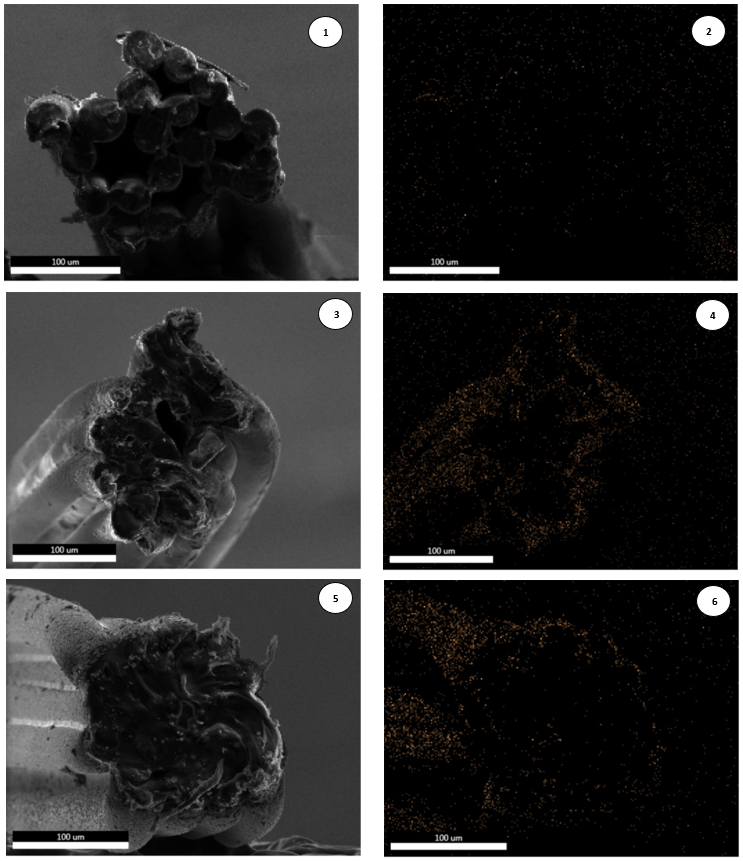
\includegraphics[width=\textwidth]{./pic/SEMAppendix.png}}
	\begin{center}
		\caption{\label{SEMAppendix} Analysis of Crosssection, left: SEM, right: EDX\\
			1) Glucose 3) \ce{NaBH4} 5) Ascorbic Acid}
	\end{center}

\end{figure}


\section{Protocols}
\label{App:Protocols}

\subsection{Sample Fabrication}

Prerequisites: \hfill\newline

\begin{multicols}{2}
	\begin{itemize}
		\item Gold concentration (\textit{c\textsubscript{gold}})
		\item Gold immersion time (\textit{t\textsubscript{gold}})
		\item Choice of reducing agent
		\item Reducing agent concentration (\textit{c\textsubscript{Red}})
		\item Reducing agent immersion time (\textit{t\textsubscript{Red}})
	\end{itemize}
\end{multicols}

\paragraph{Initial Protocol}

\begin{enumerate}
	\item Define which parameters are fixed and which are experimental parameters. Define range you want to investigate.
	
	\item Define concise naming concept, which allows every sample to be uniquely identified.
	
	\item Per sample reserve two petri dishes (PD) and label them in accordance with above mentioned concept. You might add the tag "Pre" and "Post" to existing description. (\textit{PDPre/PDPost}).
	
	\item Put 0.75ml of Gold Solution with \textit{c\textsubscript{gold}} in small, optimally non-translucent viol to account for the light-sensitivity of the gold salt (\textit{Viol}). One viol per sample you wish to investigate. Further decrease of translucency can be achieved by putting aluminium around viol.
	
	\item Put fiber in corresponding \textit{viol} and let immerse according to your defined \textit{t\textsubscript{gold}}.
	\item Take fiber out \textit{viol} and put in \textit{PDPre} to let dry. Note change in colour and/or structure. Experience shows that 30 minutes is sufficient.
	
	\item Gently pour 1ml of reducing agent solution with \textit{c\textsubscript{Red}} over fiber, while making sure the whole fiber is immersed. Note colour gradient in fiber and temporal resolution. Let immerse according to defined \textit{t\textsubscript{Red}}.
	
	\item After passing of time, transfer the fiber gently to \textit{PDPost}, where it will dry.
\end{enumerate}

\begin{center}
	This marks the end of the initial fiber fabrication.
\end{center}


\paragraph{Optimized Protocol} \hfill\newline

1. / 2. are identical to initial protocol.

\begin{enumerate}
	\setcounter{enumi}{2}
	
	\item Per sample reserve one petri dish (PD) and one glass slide (GS). Label them in accordance with above mentioned concept, whereas you might add the tag "Pre" to the PD and "Post" to GS description. (\textit{PDPre/GSPost}).
	
	\item Put 0.75ml of Gold Solution with \textit{c\textsubscript{gold}} in small, optimally non-translucent viol to account for the light-sensitivity of the gold salt (\textit{Viol}). One viol per sample you wish to investigate. Further decrease of translucency can be achieved by putting aluminum around viol.
	
	\item Put fiber in corresponding \textit{viol} and let immerse according to your defined \textit{t\textsubscript{gold}}.
	\item Take fiber out viol and put in \textit{PDPre} to let dry. Note change in color and/or structure. Experience shows that 30 minutes is sufficient.
	
	\item Gently pour 1ml of reducing agent solution over fiber, while making sure the whole fiber is immersed. Note color gradient in fiber and temporal resolution. Let immerse according to defined \textit{t\textsubscript{Red}}.
	
	\item After passing of time, transfer the fiber gently to \textit{GSPost}, where it will dry.
\end{enumerate}

\begin{center}
	This marks the end of the optimized fiber fabrication.
\end{center}

\subsection{Resistance Measurement}

\paragraph{Protocol}
\label{App:ResMeas} \hfill\newline


\begin{enumerate}
	\item Measure length of sample and write down. (=$length_{Sample}$)
	
	\item Cut the piece of paper in half, while making sure to minimally interfere with the fiber.
	
	\item Connect the both distal ends of the cable with the electrodes.
	
	\item Gently tuck the sample in the zwick.roell-tensile testing machine by making sure that the most medial border of tape is aligned with the medial border of the clamp. 
	
	\item Start gauge measurement of resistance.	
	
	\item With a slow velocity of 0.5mm/s increase the distance to achieve a more straight orientation of the sample. Stop immediately when resistance increases. Measure length between both medial ends of the two clamps and write it down.
	
	\item Abort and omit gauge measurement 
	
	\item Start now sample measurement of resistance. (= $t_{\text{StartMeasurement, 0\%}}$)
	
	\item After every 30 seconds, increase the distance between the clamps by $\frac{length_{Sample}}{100}$ with velocity 2mm/s, therefore stretching the sample by 1\%. This yields data where in the interval [0s,30s] measurements for $R_{0\%}$ is done, where $R_{0\%}$ means measured resistance of fiber with 0\% strain. Consequently, the interval [31s, 60] yields measurement of $R_{1\%}$, and so forth.
	
	\item Stop measurement when either defined maximum strain is reached, measured conductivity is implausible or conductivity is lost ($R=\infty$).
	
	\item When processing data, calculate average of all data points in interval [$t_{StartMeasurement}$ + 5s, $t_{EndMeasurement}$ - 5s], therefore eliminating inclusion of possible overshoot after increase in strain.
\end{enumerate}


\end{appendices}

